\documentclass[10pt]{report}
\usepackage{fullpage}
\usepackage{graphicx}
\usepackage{verbatim}
\usepackage{subfig}

\newcommand{\HRule}{\rule{\linewidth}{0.5mm}}

\begin{document}
\begin{titlepage}
\begin{center}
% Upper part of the page

\includegraphics[width=0.15\textwidth]{logo.jpg}\\[2cm]    
\textsc{\LARGE CS 474}\\[1.5cm]

\textsc{\Large Image Processing}\\[0.5cm]


% Title
\HRule \\[0.4cm]
{ \huge \bfseries Programming Assignment 4}\\[0.4cm]

\HRule \\[1.5cm]

% Author and supervisor
\begin{minipage}{0.4\textwidth}
\begin{center} \large
\emph{Author:}\\
Marvin \textsc{Smith}
\end{center}
\end{minipage}
\vfill
% Bottom of the page
{\large \today}
\end{center}
\end{titlepage}
\newpage

%**************************************************%
%                    INTRODUCTION                  %
%**************************************************%
\section*{Introduction}

This project is concerned with filtering in the frequency domain.
The project fulfills the following requirements\ldots\\
\begin{itemize}
\item Applying Filters in both Frequency and Spatial Domain.
\item Measure difference between filter effects using Mean Square Error.
\item Apply Homomorphic Filtering to an image and vary variables.
\item Compare effects of high-frequency filtering and histogram equalization in different orders. 
\end{itemize}

\section*{Section 1 - Gaussian Filtering}
This component requires that the program apply Gaussian filters on both the 
spatial and frequency domain. The differences will then be compared using
the Mean Squared Error.\\

In order to compare the effects of Gaussian filtering, I created a function which
produces 2D Gaussian Filters as well as 1D separable filters. The width of the 
filters is defined as $5\sigma$\\

\begin{equation}
\textup{G}_{\sigma}(x,y) = \frac{1}{2\pi\sigma^2}{\Large e}^{-\frac{x^2 + y^2}{2\sigma^2}}
\end{equation}
\begin{equation}
\textup{G}_{\sigma}(x) = \frac{1}{\sqrt{2\pi}\sigma}{\Large e}^{-1\frac{x^2}{2\sigma^2}}
\end{equation}

First, I compute the convolution using the separable filters in the spatial domain. Next, 
I compute a 2D filter of the same size as the separable filters and apply an FFT. I take the
FFT of the image, multiply the images, then compute the inverse FFT. I test various values of
$\sigma$ at $1, 1.4, 2, and 3$. To compute the difference of the images, I use the Mean Square Error.\\

\begin{equation}
\textup{MSE} = \frac{1}{MN}\sum_{x=0}^{M-1}\sum_{y=0}^{N-1}\left [ f_{\small{spatial}}(x,y)-f_{\small{frequency}}(x,y)\right ]^2
\end{equation}

\begin{figure}[!h]
\centering
\subfloat[girl.pgm]{\includegraphics[width=1.5in]{girl.jpg}}
\subfloat[lenna.pgm]{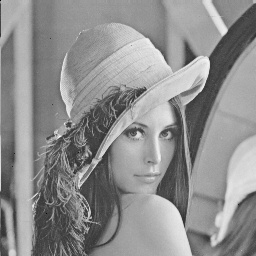
\includegraphics[width=1.5in]{lenna.jpg}}
\subfloat[boat.pgm]{\includegraphics[width=1.5in]{boat.jpg}}
\caption{Original Image}
\end{figure}

\clearpage

\begin{figure}[!h]
\centering
\subfloat[girl.pgm]{\includegraphics[width=1.5in]{girl1.jpg}}
\subfloat[lenna.pgm]{\includegraphics[width=1.5in]{lenna1.jpg}}
\subfloat[boat.pgm]{\includegraphics[width=1.5in]{boat1.jpg}}
\caption{Spatially Blurred Image at $\sigma = 2$}
\end{figure}
\begin{figure}[!h]
\centering
\subfloat[girl.pgm]{\includegraphics[width=1.5in]{girl2.jpg}}
\subfloat[lenna.pgm]{\includegraphics[width=1.5in]{lenna2.jpg}}
\subfloat[boat.pgm]{\includegraphics[width=1.5in]{boat2.jpg}}
\caption{Frequency Blurred Image at $\sigma = 2$}
\end{figure}

\begin{table}[!h]
\centering
\begin{tabular}{|l|l|l|l|}\hline
\textbf{$\sigma$} & \textbf{Diff girl.pgm} & \textbf{Diff lenna.pgm} & \textbf{Diff boat.pgm}\\\hline
$1$   & $0.505$ & $0.500$ & $0.500$ \\\hline
$1.4$ & $0.501$ & $0.504$ & $0.502$\\\hline
$2$   & $0.498$ & $0.500$ & $0.500$\\\hline
$3$   & $0.500$ & $0.500$ & $0.500$\\\hline
\end{tabular}
\caption{Differences from Mean Square Error}
\end{table}

These results show that both techniques produce the same results. The 0.5 differences that 
have been attained are most certainly from rounding errors. Due to the programming, the convolution
in the spatial domain is conducted using integer grayscale image. The convolution in the frequency domain
is conducted using floating point complex images. This makes rounding errors very delicate. Originally, errors
ranged from 4 to 50 depending on $\sigma$. After removing specific rounding and truncation errors, accuracy is
up to 0.5. There is probably something in the convolution function which rounds down due to truncation. 

\clearpage
\section*{Section 2 - Homomorphic Filtering}
Homomorphic filtering is a technique to help alleviate illumination issues such as the case in Figure \ref{fig:girl}.\\

\begin{figure}[!h]
\centering
\includegraphics[width=2in]{girl.jpg}
\caption{girl.pgm}
\label{fig:girl}
\end{figure}

Homomorphic filtering is done in this project using the following algorithm. \\
\begin{itemize}
\item Calculate $M \times M$ filter using Equation \ref{eq:homomorphic}
\item Compute FFT on Filter
\item Calculate $N \times N$ FFT on image
\item Multiply both the image and filter per-pixel
\item Compute inverse FFT
\end{itemize}

\begin{equation}
H(x,y) = \left ( \lambda_h - \lambda_l \right )\left (1 - e^{-c\frac{(x-\frac{N}{2})^2 +(y-\frac{M}{2})}{D_o^2}} \right )+\lambda_l
\label{eq:homomorphic}
\end{equation}

As there are various variables to consider, several sample images have been used.\\
\begin{figure}
\centering
\subfloat[Original]{\includegraphics[width=1.5in]{girl.jpg}}
\subfloat[$D_o=1.8$, $M=15$, $\lambda_h=8.9$, $\lambda_l=0.2$, $c=1$]{\includegraphics[width=1.5in]{girl_1.jpg}}
\subfloat[$D_o=1$, $M=15$, $\lambda_h=3$, $\lambda_l=0.2$, $c=1$]{\includegraphics[width=1.5in]{girl_2.jpg}}\\
\subfloat[$D_o=.5$, $M=15$, $\lambda_h=3$, $\lambda_l=0.1$, $c=1$]{\includegraphics[width=1.5in]{girl_3.jpg}}
\subfloat[$D_o=.5$, $M=15$, $\lambda_h=3$, $\lambda_l=0.05$, $c=1$]{\includegraphics[width=1.5in]{girl_4.jpg}}
\caption{Results with different variables}
\end{figure}

After homomorphic filtering, the image has much more clear definition. There is much more visible detail around the 
image. Where the greatest difference was noted was changing the $\lambda_l$ and $\lambda_h$. As the 
higher lambda got higher, the effect it had on the image was minimal. The lower lambda had much better results 
as it neared 0. The $D_o$ and c had almost no effect on the image. Also, the kernel size of the original filter
made a small difference as well.

\clearpage
\section*{Section 3 - Extra Credit}
The extra credit component is to show if histogram equalization and image enhancement are effective. Then, prove 
in which order.\\

To handle this, I show the result from two image tests. These test are conducted by 
applying high-boost filtering and histogram equalization in opposing orders. The results
are shown in Figure \ref{fig:ec}.\\

\begin{figure}[!h]
\centering
\subfloat[Histogram Equalization, then High Boost Filtering, A=2 ]{\includegraphics[width=1.5in]{ec1.jpg}}
\subfloat[High Boost Filtering, then Histogram Equalization, A=2 ]{\includegraphics[width=1.5in]{ec2.jpg}}\\
\subfloat[Histogram Equalization, then High Boost Filtering, A=1.5 ]{\includegraphics[width=1.5in]{ec3.jpg}}
\subfloat[High Boost Filtering, then Histogram Equalization, A=1.5 ]{\includegraphics[width=1.5in]{ec4.jpg}}
\subfloat[Histogram Equalization, then High Boost Filtering, A=4.5 ]{\includegraphics[width=1.5in]{ec5.jpg}}
\subfloat[High Boost Filtering, then Histogram Equalization, A=4.5 ]{\includegraphics[width=1.5in]{ec6.jpg}}
\caption{High Boost Filtering w/ Histogram Equalization}
\label{fig:ec}
\end{figure}

Applying image enhancement first, followed by histogram equalization is a much stronger
process. The image enhancement will bring out small details in the image, and then the 
histogram equalization will spread the range out. Histogram equalization does not try to 
destroy information, just adjust the range so that your values are more clear.\\ 

Opposite to this, using histogram equalization first will cause your image to be
washed out. The histogram equalization will center the range of pixels, then the image
enhancement will be left with small changes. Notice the gray values. 

\begin{figure}[!h]
\includegraphics[width=3in]{fig6a.jpg}
\includegraphics[width=3in]{fig6b.jpg}
\caption{Histogram Effects of Each Method}
\end{figure}

\clearpage
\section*{Conclusion and Results}
As shown this program meets the specification of the assignment sheet. I have taken from this a better understanding
of the benefits and uses of filtering in the frequency domain as compared to the spatial domain. Not only are
the results computed faster, the filters have an ability to extract more information. You are not limited by 
local information in the kernel. 


\end{document}
